\chapter{Resultados y Discusiones}
El siguiente capítulo se trabajó a base de la forma de validación detallada en el capítulo anterior. En este, también se detallan los resultados obtenidos.

\section{Detalles de resultados}
Se realizaron varias reuniones con profesores de la materia de Fundamentos de Programación, en éstas se revisaron los \textit{puzzles} del juego, se les mostró las mecánicas del juego y se revisó con ellos la forma de instalación. Esto último, dado que por falta de tiempo la instalación se hace por el docente en su propia máquina. Las reuniones se realizaron para ver las opiniones del producto realizado para usuarios finales potenciales. Los usuarios a los que tiene más potencial de afectar el juego son a los estudiantes, pero como los profesores son los que implementan el juego en su clase, es importante de primera mano un estudio para explorar sus perspectivas respecto al juego creado.

Se realizaron reuniones con cinco distintos docentes del departamento de ingeniería eléctrica y computación de la Universidad Autónoma de Ciudad Juárez que imparten o impartieron en los últimos semestres la materia de Fundamentos de Programación en el campus de Ciudad Universitaria. Posteriormente de ésta, se les realizó una pequeña encuesta sobre su parecer del juego, en diferentes aspectos entre los cuales la instalación, \textit{puzzles} y mecánicas de juego.  Se pueden ver más detalles de esta en el anexo~\ref{fig:survey}.

\subsection{Primera reunión}
Se realizó esta primera reunión el 6 de octubre del 2021. Se revisó en ésta el material del juego, se vio el valor didáctico de los diferentes \textit{puzzles} del juego y de manera menos detallada, la instalación y el \textit{gameplay}. En esta revisión del juego comento de manera positiva la variedad de los \textit{puzzles}. 

Sin embargo, mencionó que debido al diseño de los \textit{puzzles} que algunos tienen código similar a \textit{C} (subfigura~\ref{fig:for_puzzle_fail_c}), otro muy parecido a \textit{Python} (subfigura~\ref{fig:for_puzzle_fail_python}) y algunos adicionales de pseudocódigo, seria complicado para el docente usar este juego para la impartición de su clase porque ``rompería'' con lo visto en clase en algunos temas. Si el profesor tiene que explicar al estudiante que ciertos \textit{puzzles} funcionan de manera diferente a como se explicó en clase, el juego pierda valor didáctico y en el peor de los casos, podría confundir a los estudiantes. En general, comentó que usaría el juego en el salón de clases hasta que los \textit{puzzles} estén más acuerdo a la carta descriptiva.
\begin{figure}[H]
    \centering
         \begin{subfigure}{0.4\textwidth}
         \centering
         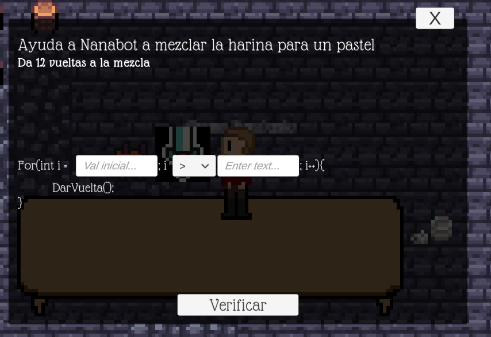
\includegraphics[width=\textwidth]{for_puzzle_fail_c}
         \caption{La sintaxis de este \textit{puzzle} era similar a C.}
         \label{fig:for_puzzle_fail_c}
    \end{subfigure}
    \begin{subfigure}{0.4\textwidth}
         \centering
         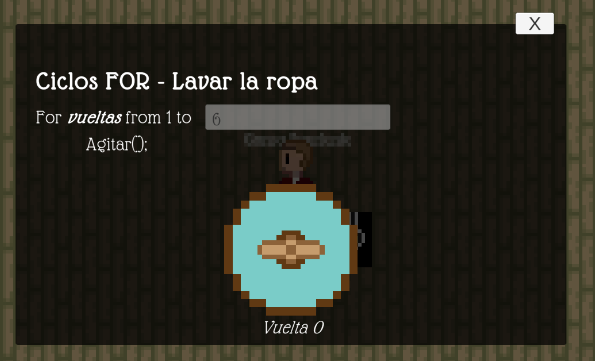
\includegraphics[width=\textwidth]{for_puzzle_fail_python}
         \caption{Este \textit{puzzle} tenía una sintaxis inspirada en \textit{Python} y su uso de \textit{ranges}.}
         \label{fig:for_puzzle_fail_python}
     \end{subfigure}
    \caption{\textit{Puzzles} que sufrieron cambios}
    \label{fig:puzzle_fail}
\end{figure}

Ante estos resultados se decidió volver a analizar el diseño y corregir los detalles encontrados en el producto para que sea posible su uso en el salón de clases. Se cambiaron los ejercicios pertinentes para usar estructuras como lo mencionan el libro  \textit{Fundamentos de programación, algoritmos, estructura de datos y objetos} de Luis Joyanes Aguilar \cite{luisjoyanesaguilar_2020_fundamentos}, que está en la carta descriptiva de la materia. Adicionalmente, se resolvió estandarizar todos los ejercicios para que usaran la sintaxis de PSeInt. 

\subsection{Segunda reunión}
Se realizó una reunión el 1 de noviembre del 2021 con otro docente. A partir de esta reunión se usaron los ejercicios rediseñados. Se le mostró los diferentes ejercicios que pueden hacer los jugadores y las mecánicas del juego.

Comentó que le pareció muy bien los \textit{puzzles}. Mencionó que los ejercicios de los ciclos y valores booleanos eran muy útiles, destacando que los ejercicios de ciclos donde el jugador tiene que decir cuantas vueltas dan, atacan un problema que ha tenido en sus clases. Adicionalmente detalló que los ejercicios de ciclos que requieren que los jugadores pongan los parámetros correctos son muy útiles porque algunos de sus estudiantes tienen problemas razonando cuando debería terminar el ciclo. Le pareció bien que los ejercicios cambiaran de valores de manera aleatoria, de manera que sea distinta cada partida del juego. 

Agregando a lo anterior, comentó positivamente de las mecánicas del juego. Mencionó que la forma en la que está el juego puede llamar la atención a los alumnos y mantenerlos interesados en jugar más.

Lo único negativo que mencionó es que le gustaría que hubiera ejercicios de arreglos y matrices.

\subsection{Tercera reunión}
El 1 de noviembre del 2021 se tuvo una tercera reunión con otro docente, éste no imparte esta clase actualmente, pero lo hizo en semestres anteriores. De la misma manera se le mostró los diferentes ejercicios que resolverán los jugadores y las mecánicas del juego.

Hizo en la reunión las siguientes observaciones de los ejercicios:
\begin{itemize}
    \item Le gustaría que hubiera más ejercicios sobre condicionales dobles.
    \item Comentó que sería bueno agregar títulos en los \textit{puzzles} denotando el tema que trata.
    \item Le gustaría que se agregaran acertijos adicionales que agreguen \textbf{ciclos para} con pasos distintos a 1. Para sacar a los estudiantes fuera de su zona de confort y tendrían la ventaja adicional de crear un modelo mental más robusto.
    \item Las indicaciones de los acertijos deben de ser más claras con lo que se pide.
    \item Quitar las funciones, porque es algo que no se cubre del todo en su clase y los estudiantes se pueden confundir.
    \item Hay algunos lugares (como en el caso de las \textit{emergencias}) que hay ejercicios no necesariamente de programación. Considera que sería mejor si estos pudieran ser también de programación. Un trabajo a futuro a considerar respecto al juego es un modo de solo programación, donde se quiten preguntas y acertijos que no tengan nada relacionado a la presentación.
\end{itemize}

Adicionalmente, detallo que los estudiantes batallan con las condicionales y los ciclos, este juego tiene el potencial de ayudarles a reforzar su aprendizaje y ayudarles a entender mejor estos temas. Mencionó que se le hace interesante este tipo de juego, y cree que los estudiantes les gustara usarlo. Agregando, menciono que le gusto la ambientación del juego.

\subsection{Cuarta reunión}
Se agendó una reunión con un cuarto docente el 3 de noviembre del 2021. 

Este docente consideró que el juego es útil para reforzar lo aprendido en la clase de Fundamentos de Programación, cumpliendo los temas de la materia. Le pareció muy bien que los ejercicios cambiaran cada partida. Además, mencionó que le gusto que los ejercicios dieran al razonamiento de que hacen los pseudocódigos del ejercicio a resolver; y que en lugar de darles instrucciones y que tengan que escribir un resultado, se les dé un resultado y tengan que evaluar si hace lo que pide las instrucciones.

Lo único que no le convenció del todo fueron la inclusión de funciones en algunos \textit{puzzles}, porque no las ve en su clase. Además, le gustaría que a futuro existiese una versión en un \textit{host}, de manera que puedan mandar a los estudiantes a una \textit{URL} y puedan acceder de esa manera el juego.

Comentó que sí usaría este juego, como repaso al final del semestre o para un examen, por la cantidad de temas que trabaja el juego.

\subsection{Quinta reunión}
Se hizo una reunión con un quinto docente el 3 de noviembre del 2021.

Comentó que les gustaría más escalones de dificultad, donde los estudiantes tengan que resolver ejercicios más complejos y en los \textit{puzzles} con \textbf{Ciclos Para} agregar ejercicios con pasos negativos y variación de los pasos.

Este docente adicionalmente, mencionó que el limite actual de 25 estudiantes quedaba corto para su salón de clases, para poder usarlo se tendría que aumentar este limite a 30 estudiantes o incluso hasta 40, por el tamaño de los grupos de clases virtuales que se realizan actualmente por la pandemia.

\section{Discusión de los resultados}
Como se había comentado anteriormente, al terminar la reunión se les pidió a los docentes que contestaran una pequeña encuesta. Ésto a fin de tener una vista neutral sobre sus opiniones respecto al juego, en esta sección se discutirán los resultados de la encuesta junto con los detalles adicionales conocidos por las reuniones con estos docentes. 

Los docentes comentaron que se les hizo interesante el juego, y mencionaron que el juego les llamará la atención a sus alumnos cuando lo jueguen por distintos motivos y esto también se puede ver en los resultados de las encuestas, respecto a los roles \textit{programador-impostor} que son cambiantes cada partida, las mecánicas del juego y el juego multijugador entre sus compañeros que son generalmente positivos en su calificación en la encuesta (figura~\ref{fig:calif_software}).

\begin{figure}[H]
    \centering
    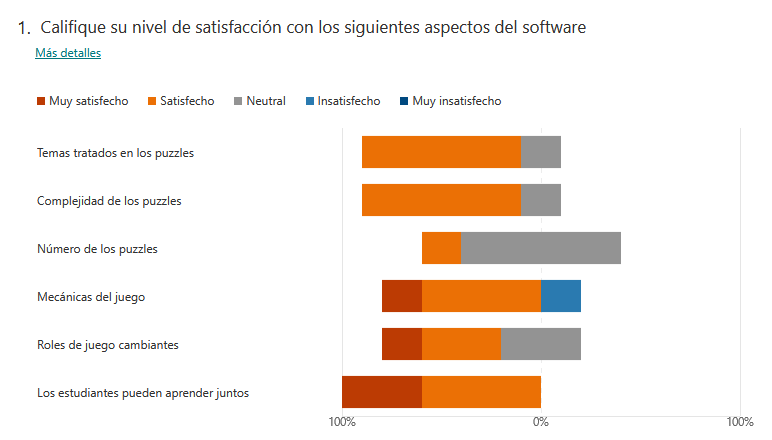
\includegraphics[width=0.8\linewidth]{images/Resencuesta (3).png}
    \caption{Calificación de satisfacción de los diferentes aspectos del producto creado.}
    \label{fig:calif_software}
\end{figure}

Sobre los \textit{puzzles}, los docentes comentaron generalmente de manera positiva de los temas tratados en los \textit{puzzles} y en cuanto a la complejidad de éstos, como se nota en la figura~\ref{fig:calif_software}. Sin embargo, no termino de convencer a los distintos docentes el número de \textit{puzzles}, sería interesante poder ver con los docentes como mejorarlo, si requieren más ejercicios o consideran que son demasiados. Después de la primera entrevista se notaron puntos débiles que limitarían la adopción del juego en el salón, esto se pudo arreglar, como se había discutido en el capítulo anterior, se cambió a la sintaxis de PSeInt para los \textit{puzzles} y se ajustaron varios de estos ejercicios para aumentar su valor didáctico. Después de estos cambios, en las reuniones les parecieron bien los ejercicios. Aunque si salieron detalles a corregir, como en algunos ejercicios el tipo de letra hace que los signos sean muy pequeños, hacer las instrucciones más claras y quitar algunas cosas en los pseudocódigos que pudiera agregar ruido a los alumnos.

Salieron algunas sugerencias adicionales, éstas son muy interesantes para explorar a futuro y agregarían valor al juego, pero no se pudieron trabajar por falta de tiempo. Entre éstas agregar temas adicionales al juego. Se les preguntó a los docentes que temas les gustaría que se agregaran al juego, arreglos estuvo en la mayoría de las sugerencias, seguido por matrices, como se puede ver en la figura~\ref{fig:temas_extras}. 

\begin{figure}[H]
    \centering
    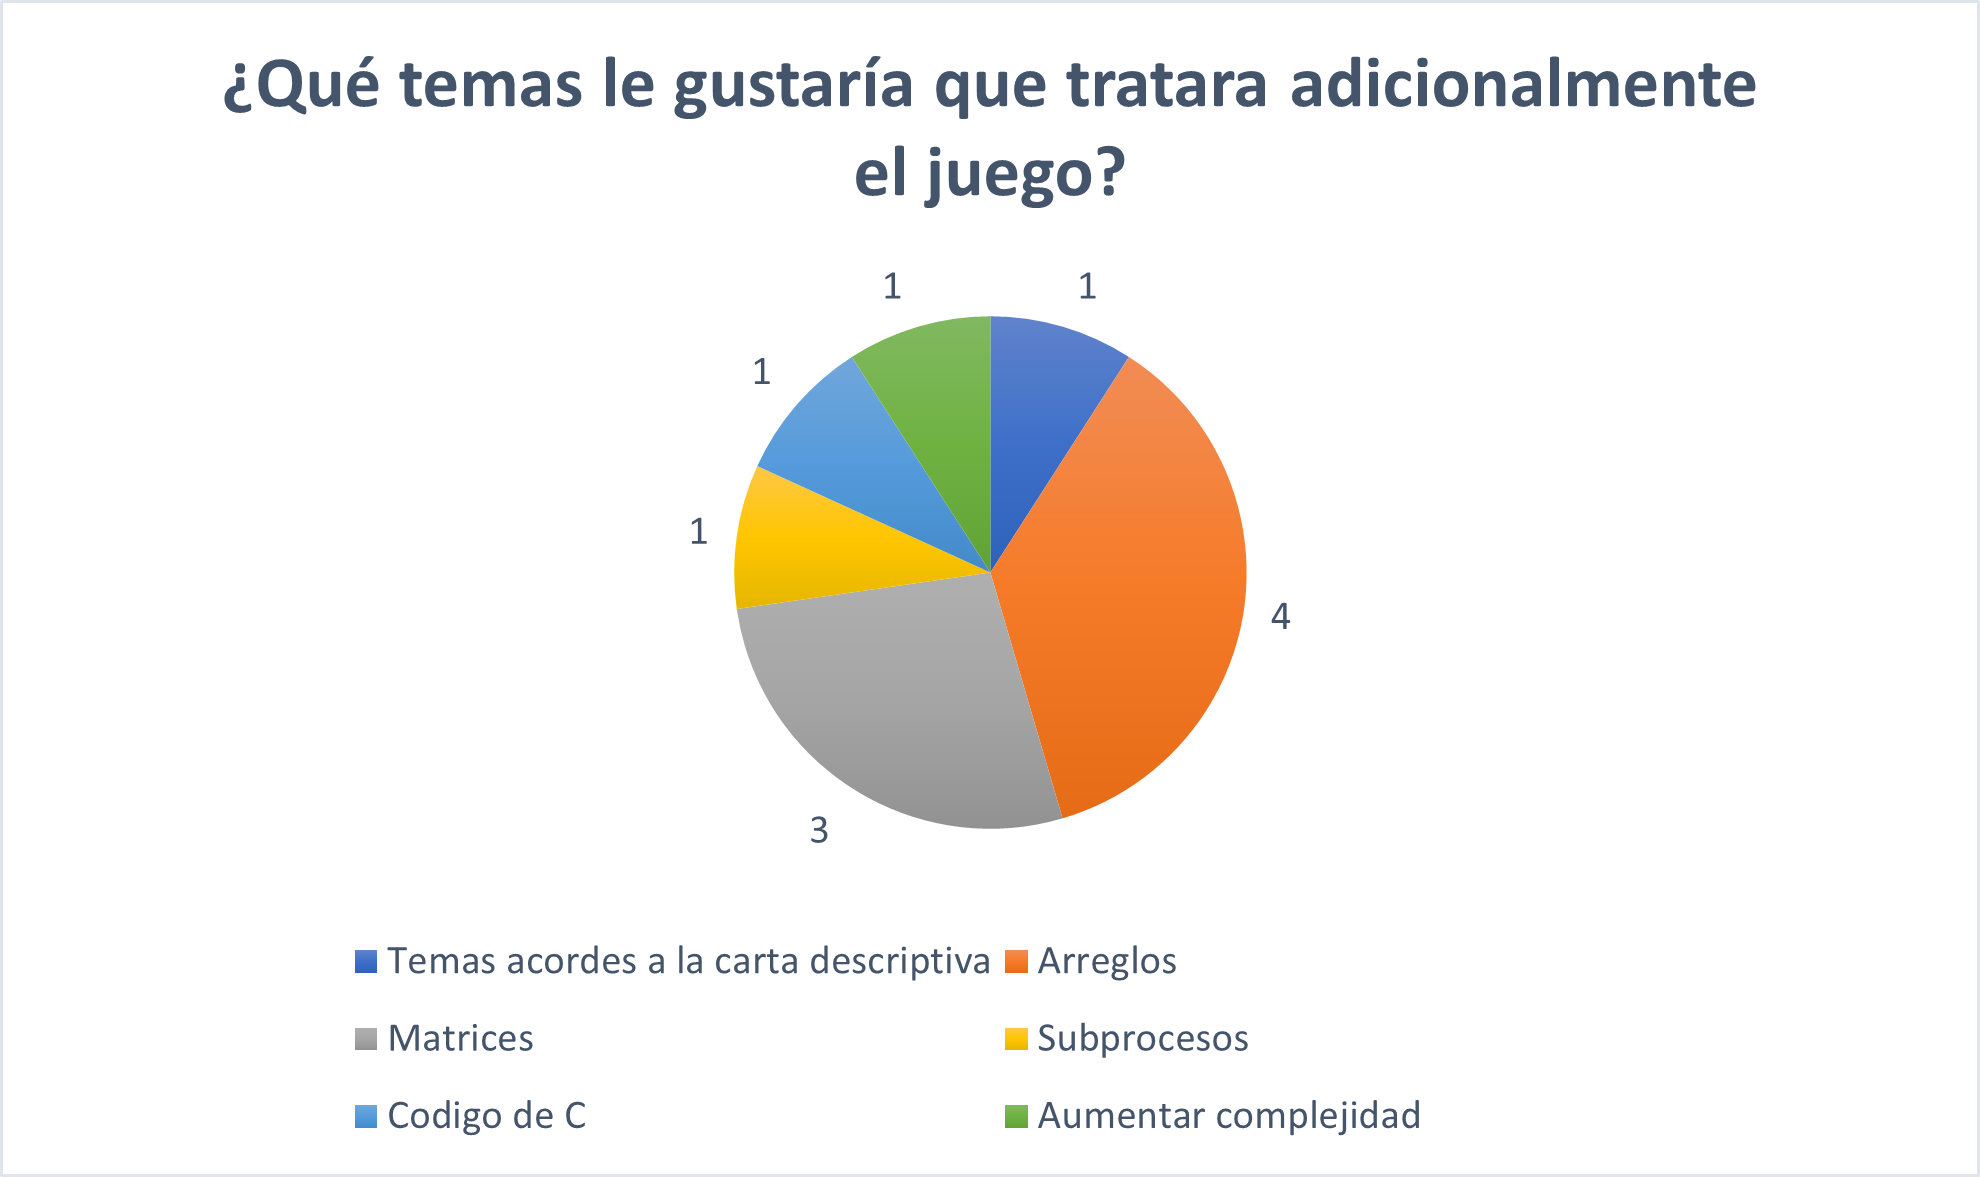
\includegraphics[width=0.8\linewidth]{images/Temas a agregar.png}
    \caption{Temas que los docentes les gustarían que se agregaran al juego.}
    \label{fig:temas_extras}
\end{figure}

El despliegue usando \textit{Docker} tiene una aceptación arriba de 7, en una escala del 0 al 10 donde 0 es nada óptimo y 10 es muy óptimo. Sin embargo, a base de las reuniones conocemos que hay sugerencias de mejora y es algo a ver a futuro para que sea más fácil de usar y expandir sus usuarios potenciales. Esto último se discutirá más adelante en trabajos futuros.

En cuanto a la probabilidad de uso del juego en el salón de clases, la opinión general de los docentes es mayormente positiva. Es muy probable a que usarían el juego en el salón de clases. En una escala del 0 al 10, donde 0 es nada probable y 10 es muy probable, cuatro docentes votaron arriba de 7. En reunión, un docente menciono que lo usaría como examen o como trabajo en clase en las ultimas semanas por los temas que trata el juego y que sus alumnos responden muy bien cuando usan software o juegos para aprender en su clase. Hubo un único resultado de 5 en este punto, por la reunión donde se planteó los cambios a los \textit{puzzles}.

Para ver con más detalle los resultados de la encuesta, éstos se puede ver en la tabla~\ref{table:resultados_survey} de la sección de anexos.
